\section{Схема установки}
\begin{figure}[H]
    \centering
    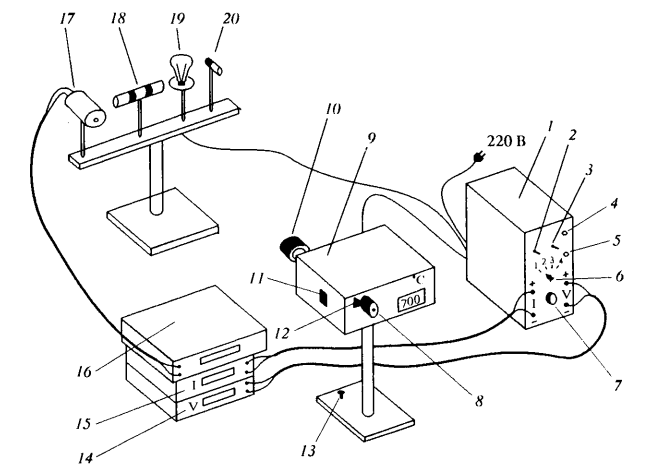
\includegraphics[width=0.6\textwidth]{img/scheme8_1.png}
    \caption{Схема установки}
    \label{fig:scheme}
\end{figure}
Экспериментальная установка состоит из оптического пирометра, модели АЧТ, образцов с общим блоком питания, а также вольтметра и амперметра для измерения тока вольфрамовой нити. Оптический пирометр с исчезающей нитью представляет собой зрительную трубу, в плоскости изображения которой находится накаливающаяся проволока. Глядя через встроенный монохроматор предполагается установить температуру проволоки такой, чтобы ее свет был <<таким же>> как свет тела, т.е. их яркостная испускательная способность сравнялась, и нить исчезла на фоне объекта. Так как прибор проградуирован по АЧТ, на экране пирометра будет отображаться яркостная температура объекта.

В качестве модели АЧТ используется керамическая трубка, нагреваемая нихромовой проволокой. Ее температура измеряется хромель-алюминиевой термопарой, подключенной к вольтметру, и позволяющей определить разность комнатной температуры с температурой АЧТ.

В качестве одного из образцов используется вольфрамовая нить лампы накаливания. Напряжение и сила тока через нее измеряются непосредственно соответствующими приборами, что даёт возможность определить ее потребляемую и излучаемую мощность. Другой образец~--- керамическая трубка с кольцами из различных материалов, нагреваемая до сравнительно однородной температуры единой нихромовой нитью. Последним изучаемым образцом является неоновая лампа.